\documentclass[ngerman]{schoolPres}

\usepackage[
  type={CC},
  modifier={by-sa},
  version={4.0},
  imagemodifier={-eu-80x15},
]{doclicense}

% --- Hier können meine Präsentationsnotizen eingeschaltet werden ---
% \setbeameroption{show only notes} % Only notes
% \setbeameroption{show notes on second screen=right} % Both

\usepackage[backend=biber, style=numeric, sorting=none]{biblatex}
\addbibresource{ref.bib}
\renewcommand*{\bibfont}{\scriptsize}

\newsavebox{\longestsec}

\date{2023-03-07}
\author{C. Badermann}
\title{Die Speicherkarte}
\subtitle{Kompakter Speicher mit großem Potenzial; der vertraute Gefährte der Datenaggregation}

\begin{document}
  \Large

  \section{Prolog}%
  \subsection{Titelfolie}%
  \begin{frame}
    \maketitle~\\

    \begin{center}
      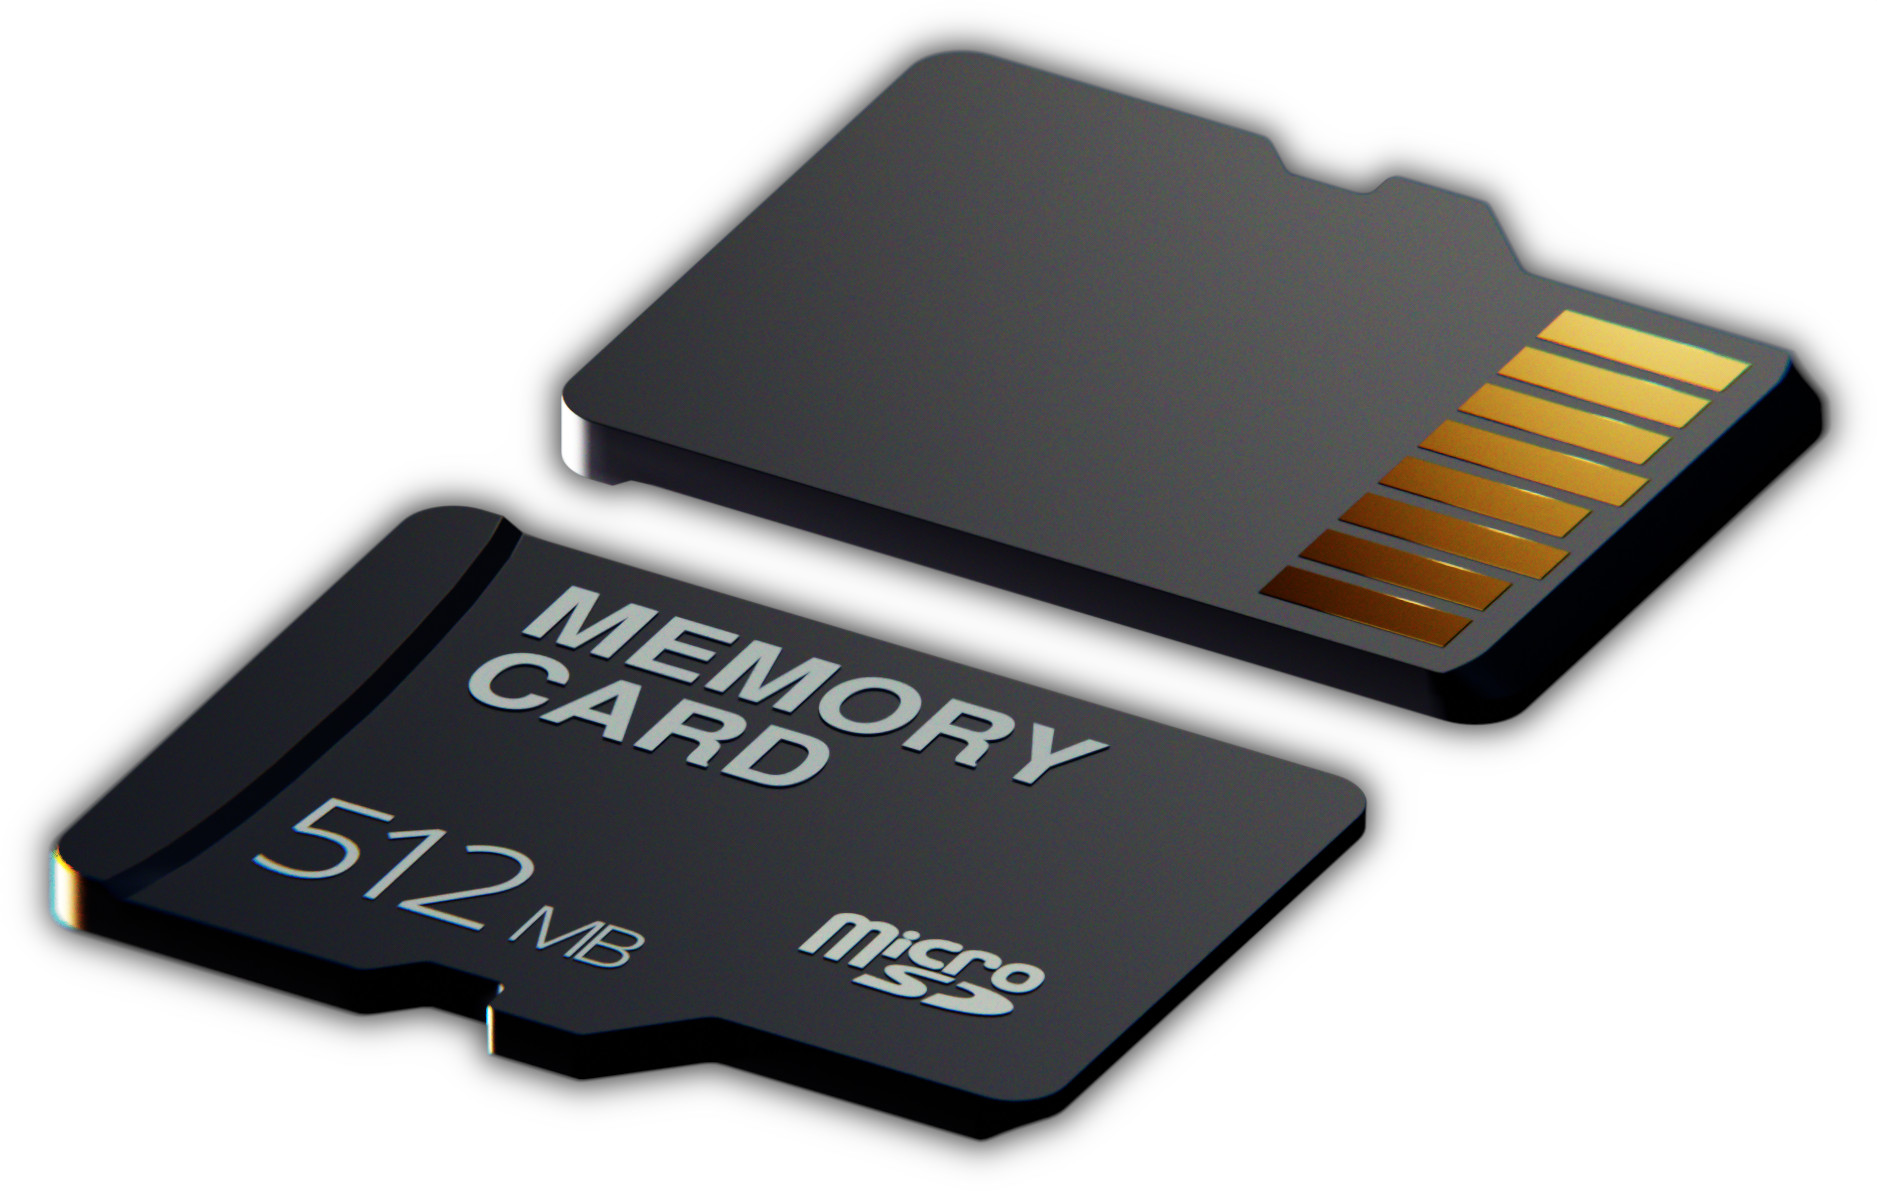
\includegraphics[height=8em]{media/title_edit.jpg}
    \end{center}
  \end{frame}

  \subsection{Inhaltsverzeichnis}%
  \begin{frame}
    % interline spacing is broken here, but I can't figure out how to fix :wah:
    % this is why nesting hacks is generally a bad idea
    \begin{multicols}{2}
      \setcounter{tocdepth}{1}
      \begin{lrbox}{\longestsec}Beispiel Projekt\end{lrbox}% Capture longest title
      \setlength{\leftskip}{\dimexpr.5\linewidth-.5\wd\longestsec\relax}
      \setlength{\lineskiplimit}{-200pt}
      \tableofcontents
      \setcounter{tocdepth}{3}
    \end{multicols}

    \note{
      - Motivation \& Einleitung der microSD-Karte\\
      - Hardware-Aspekt\\
      - Software-Lösungen (ordnungsgemäße Formatierung, Bibliotheken und deren Funktionen)\\
      - Beispielprojekt (Konstruktion nach Beschreibung, Software Design \& Programmierung, Datenanalyse)
    }
  \end{frame}

  \FramedSection{Die SD-Karte}%
  \subsection{Motivation}%
  \begin{frame}<1,2>[label=motivation]
    \usebeamercolor[fg]{structure}
    \only<3>{
      \begin{center}
        \textbf{Zur Erinnerung:}
      \end{center}
    }
    \usebeamercolor[fg]{normal text}

    \only<1>{\textbf{Szenario:}\\}
    \only<1,3>{
      Eine Wetterstation soll konstruiert werden:\\
      Messung von Temperatur, Luftfeuchtigkeit und Luftdruck, mithilfe der \enquote{\texttt{HDC100x}} und \enquote{\texttt{BMP280}} Sensoren;
      Auswertung aggregierter Daten am Computer\cite{EnergyLab-Wettermessstation}.
    }
    \only<1>{\note{
      Szenario:\\
      Wettermessstation, Aggregation auf Speichermedium, Auswertung am PC.\\~\\
    }}

    \only<2>{\textbf{Erwünschte Fähigkeiten des Speichermediums:}
    \begin{itemize}
      \item Nichtflüchtige \& alleinstehende Speicherung
      \item Einfacher Transfer von Daten auf andere Systeme
      \item Großes Speichervolumen
    \end{itemize}
    \note{
      - Nichtflüchtigkeit! (RAM / ROM)\\
      - Alleinstehend (ohne externe Systeme)\\
      - Großes Speichervolumen
    }}
  \end{frame}

  \subsection{SD \& SDA}%
  \begin{frame}
    Ein geeignetes Medium für dieses Szenario: die microSD-Karte:\\
    \tsec{(\href{https://de.wikipedia.org/wiki/Flash-Speicher}{Flash-EEPROM} nach Standard der \enquote{SD Association})}\\~\\

    \textbf{Qualitäten:}
    \begin{itemize}
      \item Kostengünstig
      \item Allgegenwärtig
      \item Kompakter Formfaktor
      \item Simple SPI Schnittstelle
      \item Müheloses Einführen, Entfernen
      \item Verfügbarkeit von Anschlüssen für Arduino und andere Systeme
    \end{itemize}

    \note {
      microSD-Karten sind cool! Yay\\

      Viele tolle Eigenschaften...
    }

    \blfootnote{\citeauthor{sd-overview} -- \enquote{\citetitle{sd-overview}}\cite{sd-overview}.}
  \end{frame}

  \begin{frame}
    SD-Karten ermöglichen die nichtflüchtige Speicherung von Daten.
    Diese sind als Dateien in einem Ordnersystem organisiert.\\~\\

    \textbf{Obacht:}
    \begin{itemize}
      \item Der Arduino unterstützt nur bestimmte Karten\cite{sd-lib}
      \item Flash-Speicher verfügt über endlich viele Schreibzyklen\cite{zhang2017flash,sd-lifespan}
      \item SD-Karten sind leicht zu verlegen und entwenden
      \item Es gibt leistungsfähigeren Speicher
      \item SD ist ein proprietärer Standard\cite{sd-proprietary}
    \end{itemize}

    \note {
      Es gibt einiges zu beachten...
    }
  \end{frame}

  \FramedSection{Hardware}%
  \subsection{SD-Karten}%
  \begin{frame}
    \begin{columns}[c]
      \begin{column}{.6\linewidth}
        Ein Standard der \enquote{SD Association} bestimmt welche Karten unter dem \emph{SD} Warenzeichen verkauft werden dürfen.\\~\\

        Im inneren sind Flash-Speicher, sowie ein Mikrocontroller zu finden.
      \end{column}
      \begin{column}{.4\linewidth}
        \begin{figure}[!ht]
          \centering
          \begin{subfigure}{.65\linewidth}
            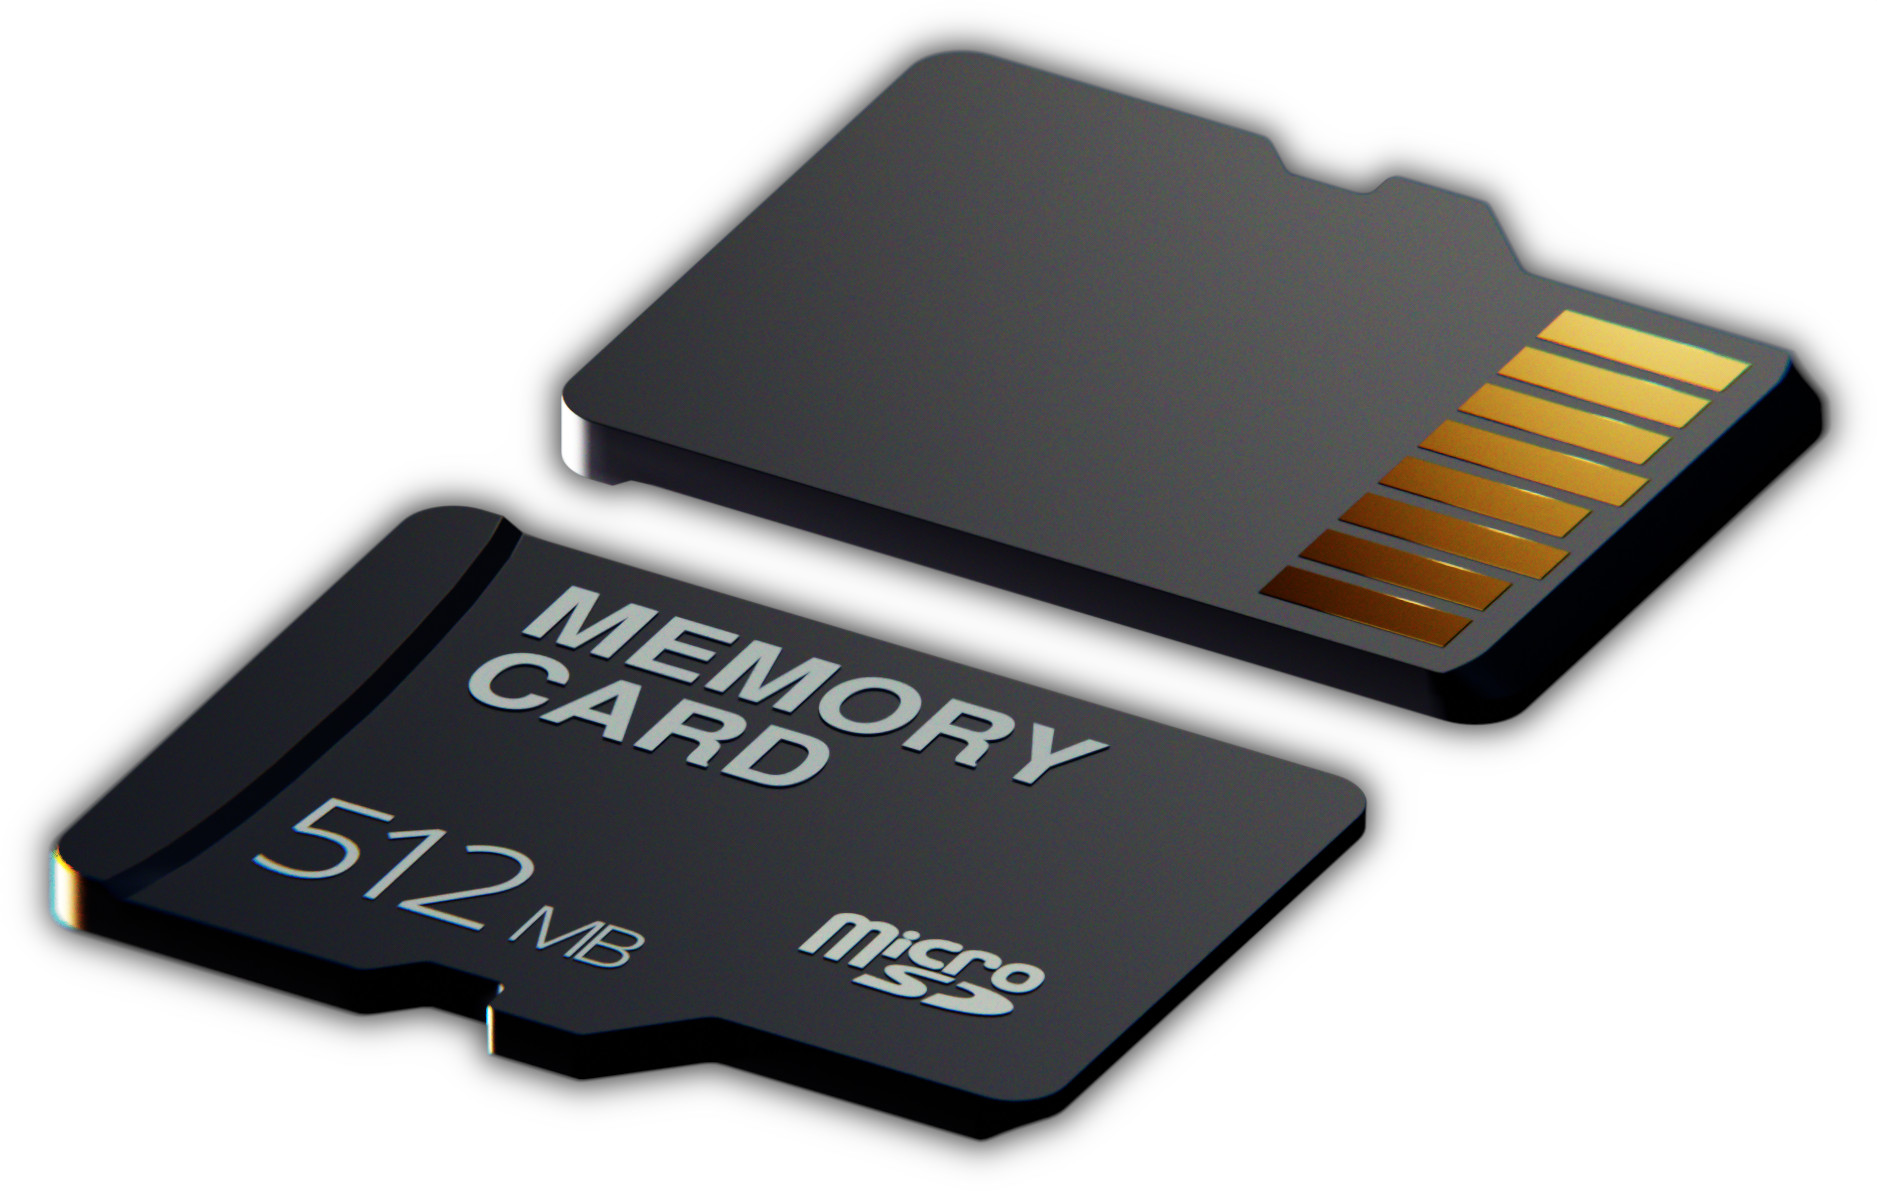
\includegraphics[width=\linewidth]{media/title_edit.jpg}
          \end{subfigure}\vspace{1em}

          \begin{subfigure}{.3\linewidth}
            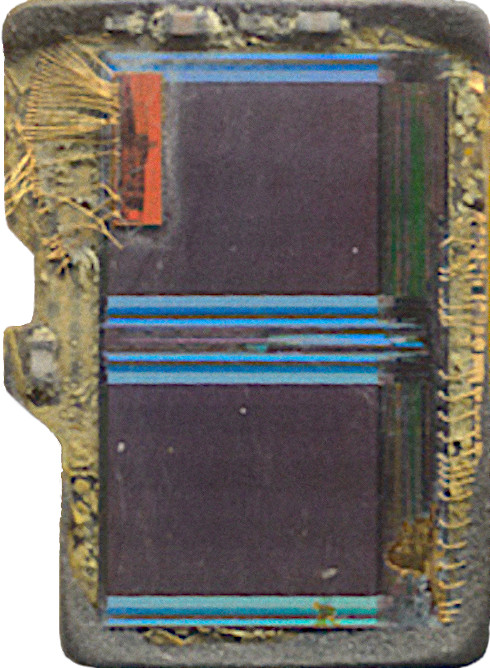
\includegraphics[width=\linewidth]{media/decapsulated-01.jpg}
            \caption{\tiny \href{https://commons.wikimedia.org/wiki/File:Decapsulated\_microSD\_memory\_card\_lineup-genuine,\_questionable,\_and\_fake-counterfeit.jpg}{Huang -\\CC BY-SA 3.0}}
          \end{subfigure}\hspace{4em}
          \begin{subfigure}{.3\linewidth}
            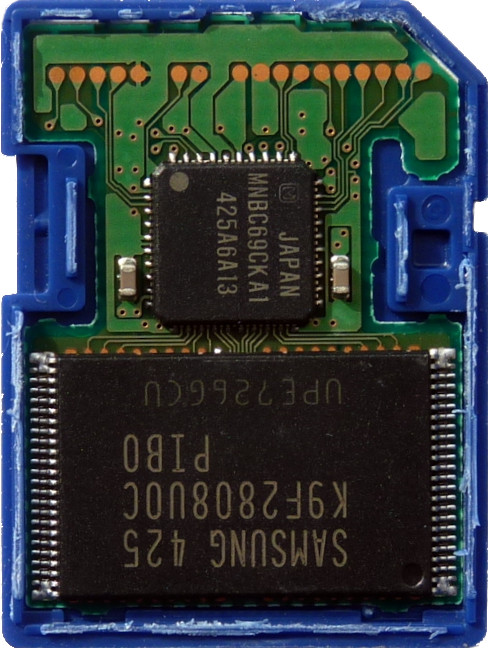
\includegraphics[width=\linewidth]{media/decapsulated-02.jpg}
            \caption{\tiny \href{https://commons.wikimedia.org/wiki/File:SDKarteoffen.jpg}{Jörn -\\CC BY 3.0}}
          \end{subfigure}
        \end{figure}
      \end{column}
    \end{columns}

    \blfootnote{\citeauthor{sd-spec_physical-layer} -- \enquote{\citetitle{sd-spec_physical-layer}}\cite{sd-spec_physical-layer}.}
    \note {
      Hardware definiert durch spec der SDA; SD Trademark sichert ab.\\~\\

      Innenleben: Flash-Speicher \& Mikrocontroller.\\
      Letzterer stellt nutzerfreundliche Protokolle zur strukturierten Nutzung des Speichers zur Verfügung.
    }
  \end{frame}

  \subsection{Interfaces}%
  \begin{frame}
    Schnittstellen sind häufig Shields oder Breakout-Boards.\\
    Durch beide werden Karten an den SPI-Bus angehangen.\\~\\

    \begin{figure}[!ht]
      \centering
      \begin{subfigure}{.3\linewidth}
        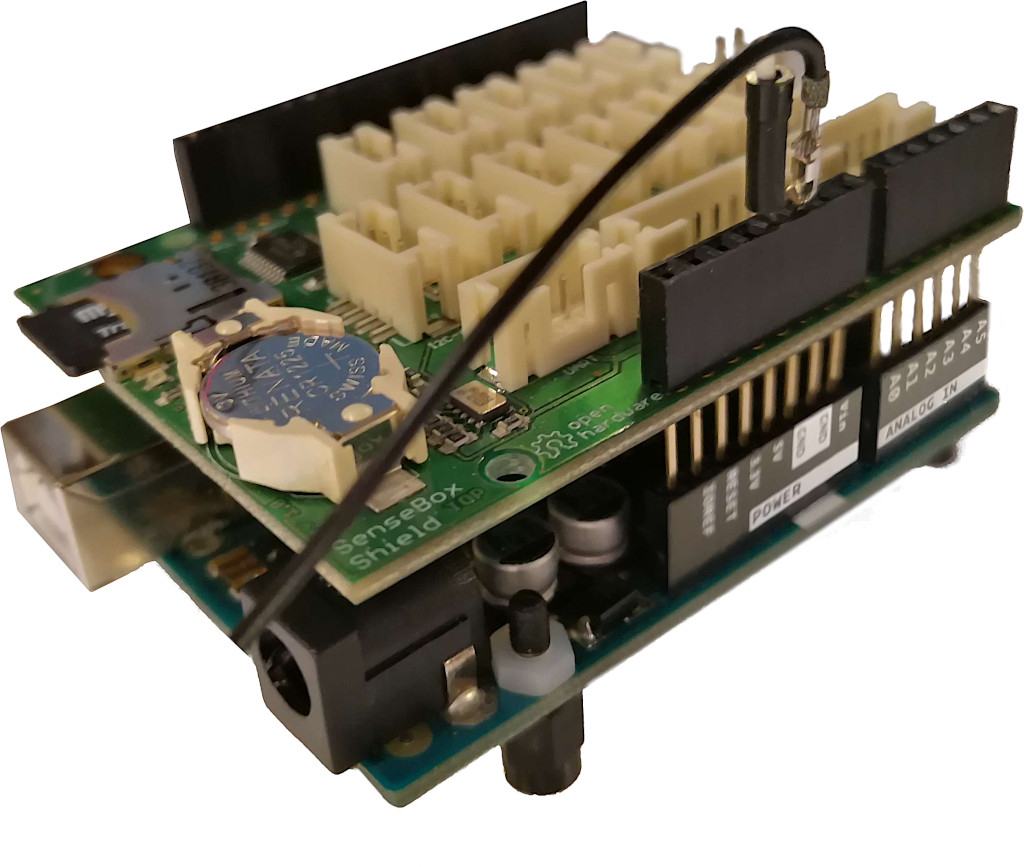
\includegraphics[width=\linewidth]{media/shield.jpg}
        \caption{\tiny Shield mit microSD Anschluss}
      \end{subfigure}\hspace{4em}
      \begin{subfigure}{.3\linewidth}
        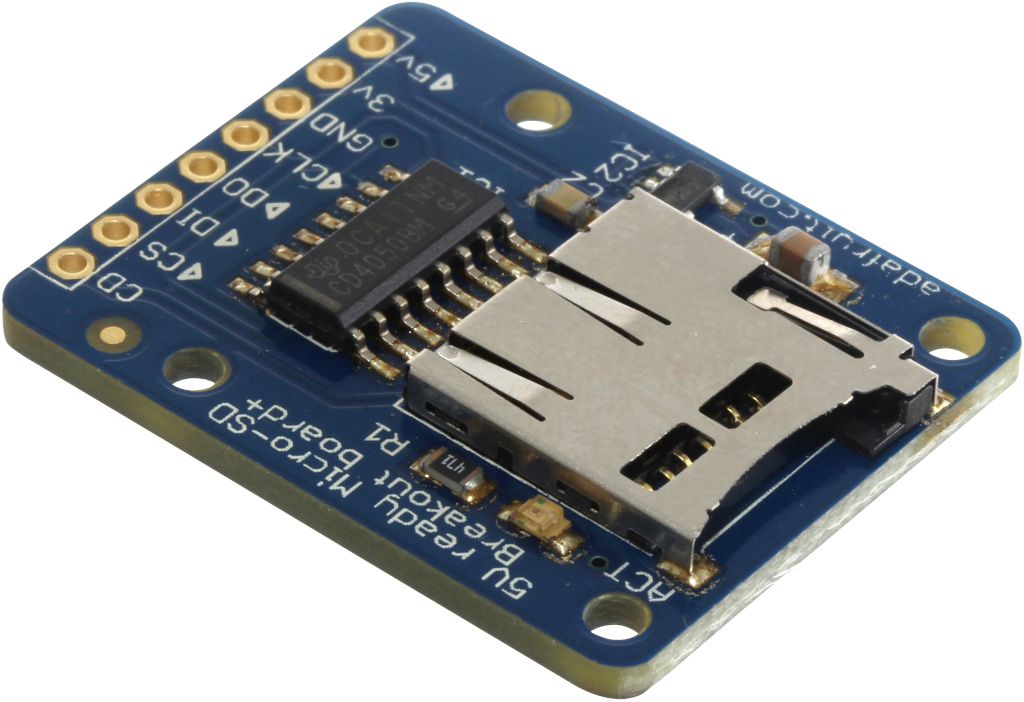
\includegraphics[width=\linewidth]{media/sd-breakout.jpg}
        \caption{\tiny microSD breakout board\\(\href{https://www.flickr.com/photos/snazzyguy/6234676208/}{oomlout, CC BY-SA 2.0})}
      \end{subfigure}
    \end{figure}

    \note {
      Schnittstellen: Shields \& Breakout-Boards.\\
      Beide per SPI-Bus.
    }
  \end{frame}

  \FramedSection{Software}%
  \subsection{SD-Karte}%
  \begin{frame}
    Zur Verwendung müssen microSD-Karten ggf. formatiert werden.
    Unterstützt sind MBR / GUID Partitionstabellen mit FAT-16 / 32 Dateisystemen\cite{sd-lib}.\\~\\

    Es wird auch SD-Bus, UHS-II Bus, oder PCIe, anstelle von SPI verwendet.
    Bestimmte Konfigurationen des SD Standards können deshalb nicht verwendet werden\cite{sd-spec_physical-layer}.

    \note {
      Speichermedium-Formatierung ist ggf. notwendig.\\
      SD-Bus Umstände.
    }
  \end{frame}

  \subsection{SD Library}%
  \begin{frame}
    SD-Library zur Verwendung von SD-Karten.\\
    Installation per Library Manager, Einbindung als \enquote{\texttt{SD.h}}.
    Zur Kommunikation per SPI-Bus wird ebenfalls \enquote{\texttt{SPI.h}} benötigt.\\~\\

    \note {
      SD Library (\texttt{SD.h} \& \texttt{SPI.h}); Installation in IDE 1.x \& 2.x.
    }

    \begin{figure}[!ht]
      \centering%
      \begin{subfigure}{.72\linewidth}
        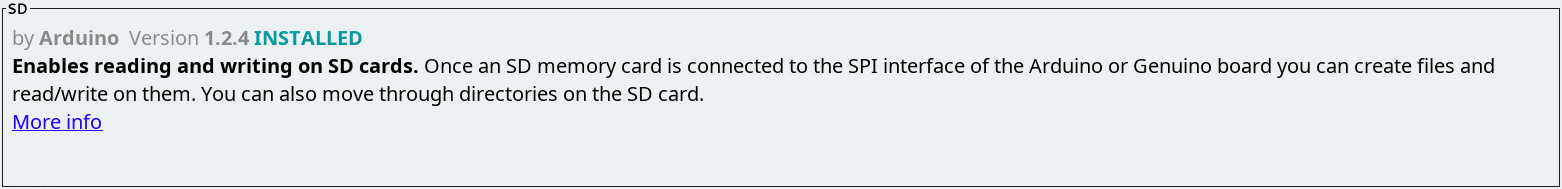
\includegraphics[width=\linewidth]{media/sd-lib.png}
        \caption{Arduino IDE 1.8}%
      \end{subfigure}\hspace{1.5em}%
      \begin{subfigure}{.2\linewidth}%
        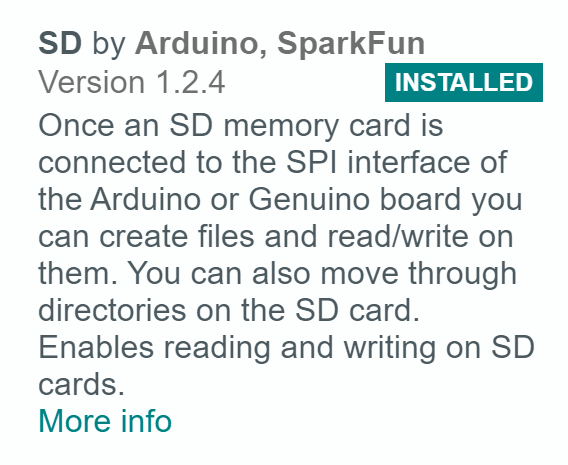
\includegraphics[width=\linewidth]{media/sd-lib-ide2.png}
        \caption{Arduino IDE 2.0}
      \end{subfigure}
    \end{figure}
  \end{frame}

  \begin{frame}[fragile]
    Durch \enquote{\texttt{SD.begin(int cs)}} wird die SPI-Verbindung hergestellt \tsec{(\texttt{cs} = \enquote{Chip-Select Pin})}.
    Dies liefert einen Boolean (1 / 0);\\Per If-Abfrage können Nutzer informiert werden.\\~\\

    \note {
      Inklusion von \texttt{SPI.h} \& \texttt{SD.h}.\\
      Herstellung der SPI-Verbindung mit Error Handling.
    }

    \lstinputlisting{./media/sketch/sd-setup.ino}
  \end{frame}

  \begin{frame}[fragile]
    \only<1> {
      Dateien sind idiomatische Container für Daten.\\
      \enquote{\texttt{SD.open(pfad, modus)}} liefert das \texttt{File} Objekt, welches zur Bearbeitung dieser benötigt wird.

      \note {
        Dateien als Container.\\
        Öffnung dieser \& \texttt{File} Objekt.
      }
    }

    \only<2> {
      Modi beschreiben welche Aktionen auf die geöffnete Datei ausgeführt werden können:\\~\\

      \note {
        Öffungs-Modi und deren Funktion. (FILE\_READ, FILE\_WRITE)\\~\\

        ggf. Attribute (\texttt{FILE\_WRITE} = (\texttt{O\_READ} | \texttt{O\_WRITE} | \texttt{O\_CREAT} | \texttt{O\_APPEND}))\\
        \enquote{\texttt{uint8\_t const O\_READ = 0X01;}}, \enquote{\texttt{uint8\_t const O\_APPEND = 0X04;}}.\\
        (\texttt{O\_READ} | \texttt{O\_APPEND} = 0x01 (0b001) | 0x04 (0b100) = 0x05 (0b101))\\
        (mehr in \texttt{SD.h} \& \texttt{SdFat.h})
      }
    }

    \only<3> {
      Interaktion mit Inhalten durch \texttt{print()}, \texttt{write()}, \texttt{read()} Befehle.\\~\\

      \note {
        Schreiben und Lesen von Daten.
      }
    }

    ~

    \lstinputlisting{./media/sketch/sd-file.ino}
  \end{frame}

  \begin{frame}
    Bearbeitung des Dateisystems durch \texttt{open()}, \texttt{mkdir()}, \texttt{rmdir()}, \texttt{remove()}.\\~\\

    Ertastung bestehender Strukturen durch \texttt{exists()}, \texttt{isDirectory()} \& \texttt{name()}.\\~\\

    Navigation via \texttt{open()}, \texttt{openNextFile()}, \texttt{rewindDirectory()}. \tsec{(\enquote{\texttt{open}} Funktionen sind ebenfalls für Ordner geeignet)}

    \note {
      Dateisystemmanagement\\~\\

      Ertasten des Dateisystems\\~\\

      Navigation des Dateisystems
    }
  \end{frame}

  \begin{frame}
    \textbf{Obacht:}\\~\\

    \texttt{File} ist gepuffert; Es können Änderungen verloren gehen.\\
    \tsec{Änderungen werden erst bei \texttt{flush} Ereignissen geschrieben.
    Dies geschieht z.B.: durch \texttt{flush()} oder das Schließen einer Datei.}\\~\\

    Versionsbedingt ist ggf. nur eine Datei an einem Zeitpunkt zu öffnen. Das Schließen sollte nicht vergessen werden.\\~\\

    \tsec{Unterstützt sind lediglich \href{https://de.wikipedia.org/wiki/8.3}{8.3 Dateinamen} in Großbuchstaben\cite{sd-lib}.}

    \note {
      \textbf{Zu beachten:}\\~\\

      \hspace{2em}File muss geflushed werden. Sonst können daten verloren gehen :/\\~\\

      \hspace{2em}\enquote{\texttt{SD.h}} kann ggf. nur eine Datei öffnen.\\~\\

      \hspace{2em}8.3 Dateinamen \& Diskrepanz zur Schreibweise des c \texttt{FILE} Objekt.
    }
  \end{frame}

  \FramedSection{Beispiel Projekt}%
  \hypertarget{sec:project}{}
  \subsection{Rückblick, Projektbeschreibung}%
  \againframe<3>{motivation}

  \subsection{Konstruktion}%
  \begin{frame}
    \begin{columns}[c]
      \begin{column}{.5\linewidth}
        Auf dem Arduino ist das \enquote{senseBox Shield} montiert.
        \tsec{Es stellt eine Echtzeituhr (\href{https://de.wikipedia.org/wiki/Echtzeituhr}{RTC}) und den microSD Anschluss bereit.}\\~\\

        Besagte Sensormodule sind über die Steckplatine an den SPI-Bus angehangen.
      \end{column}
      \begin{column}{.5\linewidth}
        \centering
        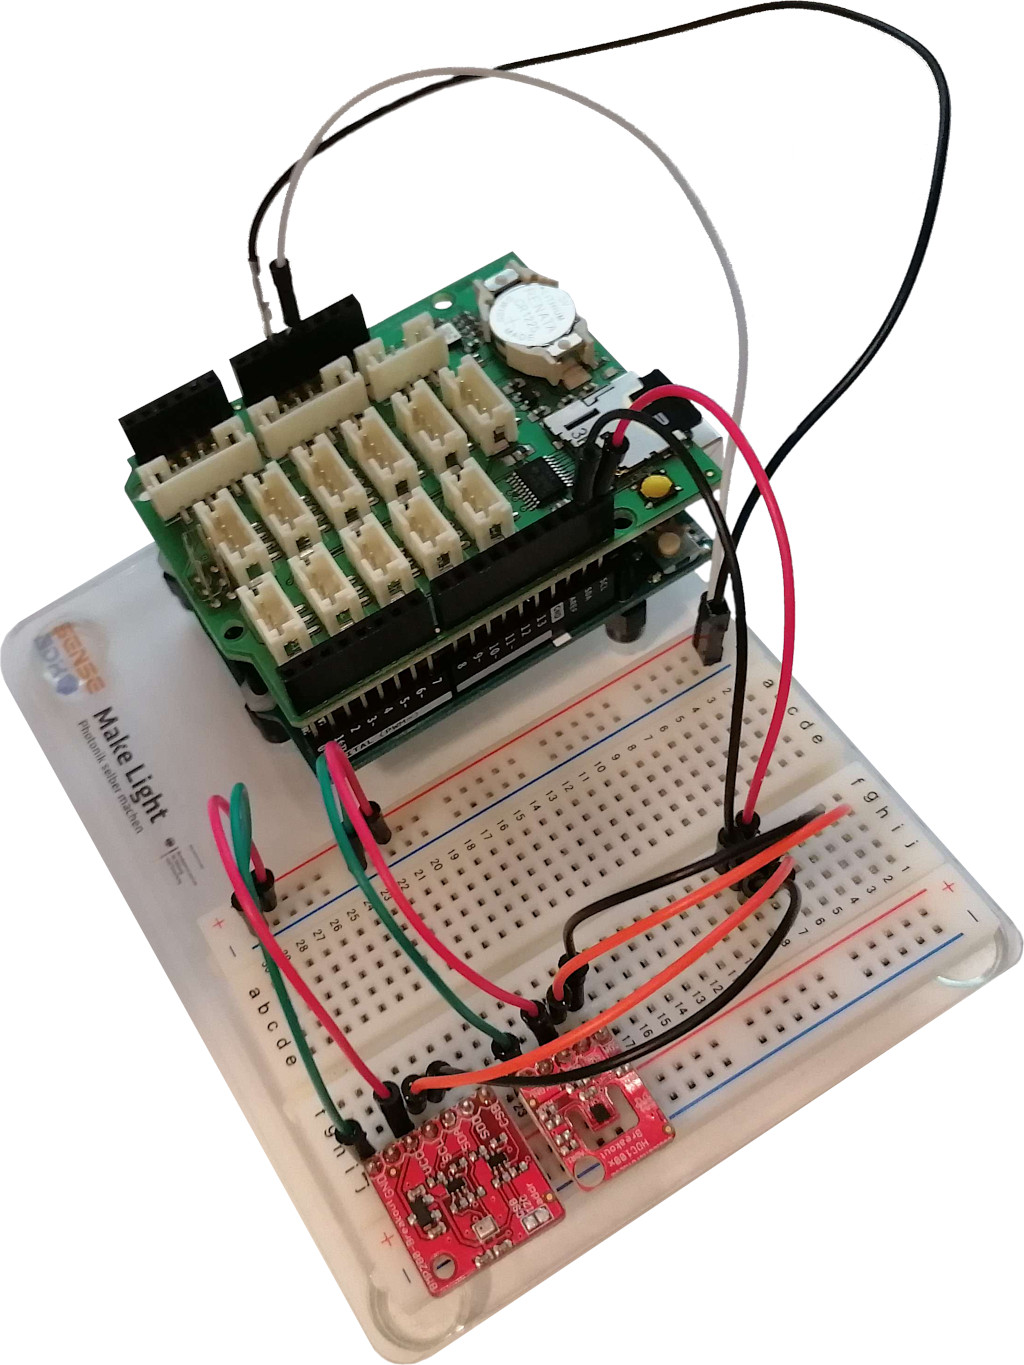
\includegraphics[height=.8\textheight]{media/board.jpg}
      \end{column}
    \end{columns}

    \note {
      Shield mit RTC und microSD Anschluss.\\~\\

      Sensoren am SPI-Bus.
    }
  \end{frame}

  \subsection{Speicherformate}%
  \begin{frame}
    \begin{minipage}{.8\linewidth}
    Die Strukturierung von Daten ist ein wichtiger Aspekt.\\
    \tsec{Textbasierte Formate sind nutzerfreundlich; Strukturierung erleichtert die Weiterverarbeitung.}\\~\\

    Menschliche sowie technische Fehler passieren.\\
    Es sollten stets Sicherheitskopien existieren\cite{chervenak-backup}.
    \end{minipage}\begin{minipage}{.2\textwidth}
      \centering
      \vfill
      
\includegraphics[width=.5\linewidth]{./media/file.pdf}
      \vfill
    \end{minipage}

    \note{
      Textbasierte Formate sind Nutzerfreundlich, Strukturierung cool für Computer.\\~\\

      Beispiel Sicherheitskopien:\\
      \hspace{2em} Jemand löscht den gesamten Datensatz des Projekts, beim Versuch diesen auszuwerten.
    }
  \end{frame}

  \begin{frame}[fragile]
    Es wurde das CSV Format gewählt\footnote{RFC 4180: \enquote{\citetitle{rfc4180}}\cite{rfc4180}.}.\\
    Als textbasiertes Format Plattform-unabhängig; tabellarisch.\\~\\

    Zeilen sind durch den Zeilenumbruch \enquote{\texttt{\textbackslash n}} oder \enquote{\texttt{\textbackslash r\textbackslash n}} getrennt.\\
    Datenfelder / Spalten durch das Komma \enquote{\texttt{,}}.\\~\\

    \lstinputlisting[caption={Beispiel CSV-Datei: (\href{https://de.wikipedia.org/w/index.php?title=CSV_(Dateiformat)\&oldid=229431469\#Beispiel}{Wikipedia -- CC BY-SA 3.0})}]{./media/sketch/csv.csv}

    \note {
      Wahl von CSV, erklärung:\\~\\

      Textbasiert \& plattform-unabhängig; tabellarisch.\\
      Trennung durch \enquote{\texttt{,}} \&  Zeilenumbruchsequenz: LF (\texttt{\textbackslash n}) / CR LF (\texttt{\textbackslash r \textbackslash n}).
    }
  \end{frame}

  \subsection{Programmierung}
  \begin{frame}[fragile]
    Libraries werden eingebunden und Sensoren definiert.\\
    \lstinputlisting{./media/sketch/include.ino}
    \note{
      Jeglicher Quelltext ist symbolisch zu Betrachten!\\
      Es sind nur Ausschnitte.\\~\\

      Einbindung der Libraries, Definition \& Initialisierung der Sensoren (dies und deren Nutzung ist immer ähnlich).
    }
  \end{frame}

  \begin{frame}[fragile]
    In \texttt{setup()} werden SPI-Verbindungen initialisiert.\\
    \lstinputlisting{./media/sketch/setup.ino}

     \note {
       SPI-Verbindung \& Error-Handling
     }
  \end{frame}

  \begin{frame}[fragile]
    In \texttt{loop()} werden Sensoren eingelesen und in den Logger gegeben.\\
    \lstinputlisting{./media/sketch/loop.ino}
    \note{
      \enquote{logger} ist eine Methode zur Datenaggregation. Jeder Aufruf wird an SD und Serial weitergegeben.
    }
  \end{frame}

  \begin{frame}[fragile]
    Die Ausgabe des Loggers:\\
    \lstinputlisting{./media/sketch/out.txt}
  \end{frame}

  \subsection{Auswertung}
  \begin{frame}
    Auswertungsbeispiel:\\~\\

    Luftdruck steht in negativer Beziehung zu Temperatur und Luftfeuchtigkeit, welche zunächst gesunken sind, sich graduell wieder den Ausgangswerten näherten.

    \begin{center}
      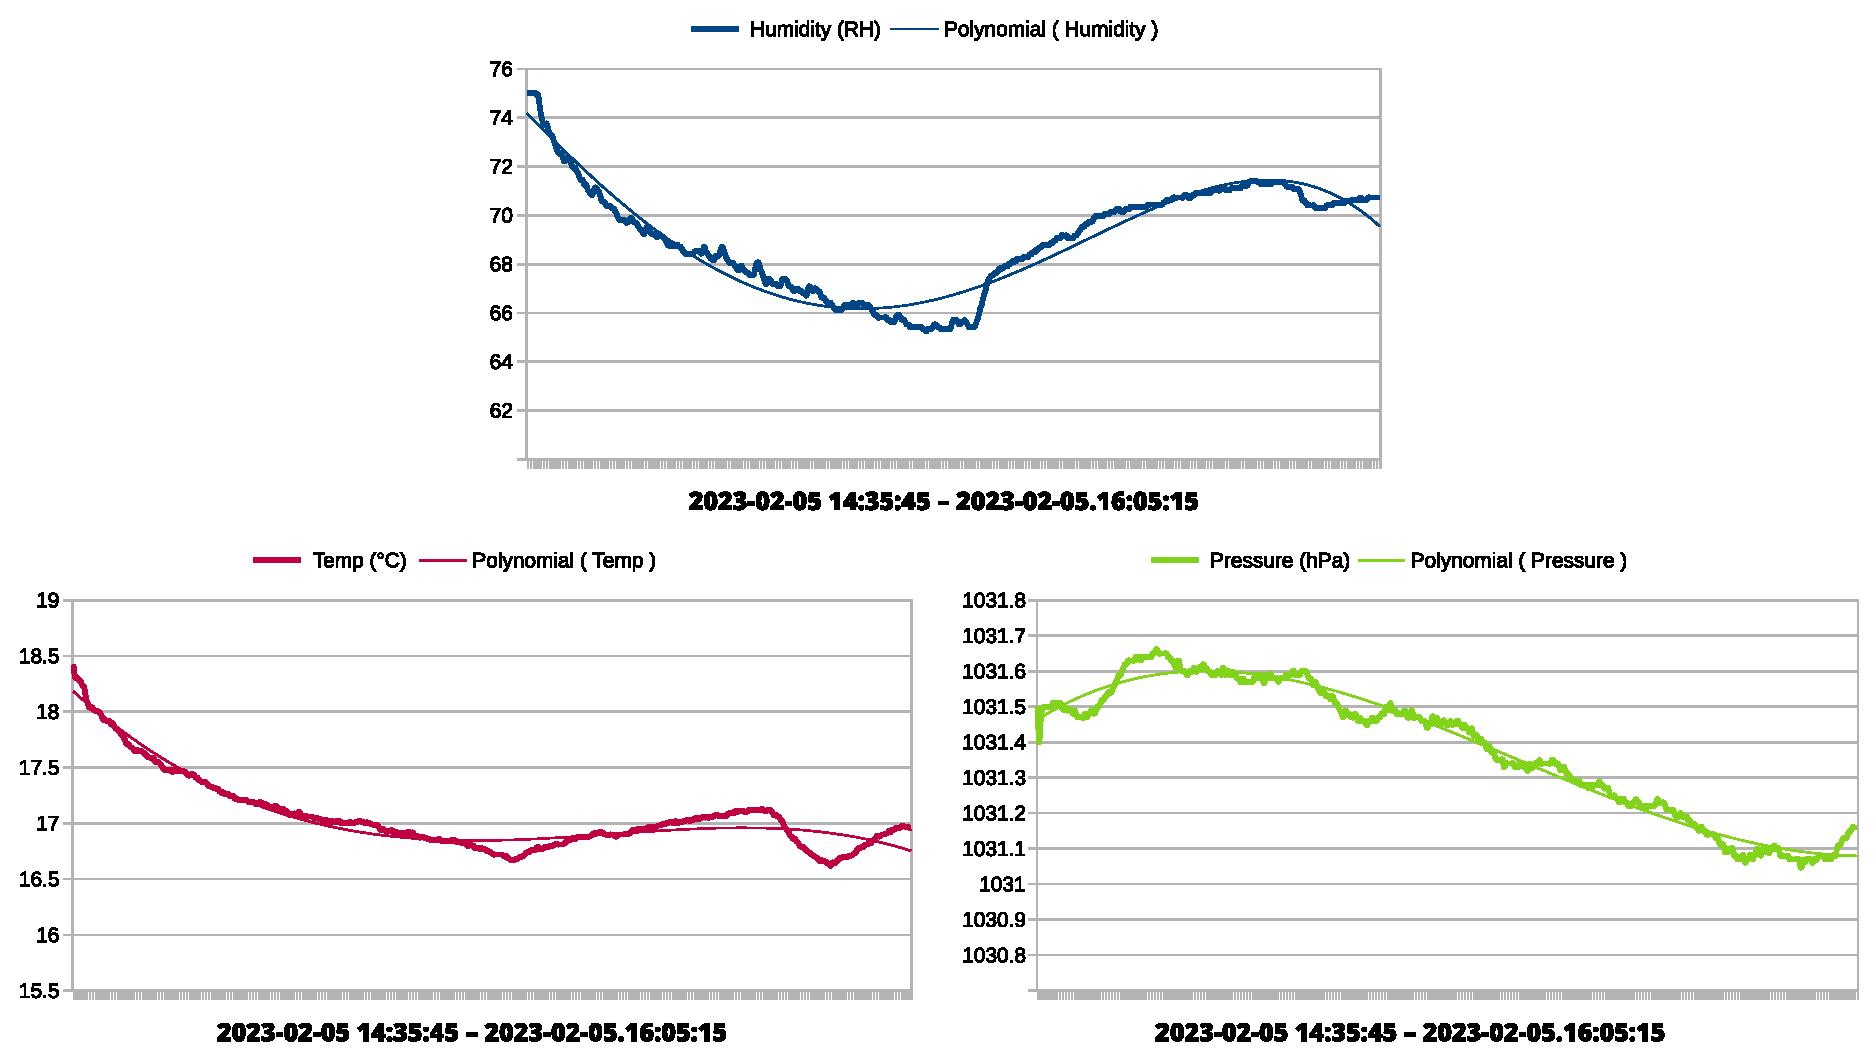
\includegraphics[width=0.5\textwidth]{media/data.pdf}
    \end{center}

    \note{
      Auswertungsbeispiel:\\~\\

      Variationen durch Öffnung eines Fensters.\\
      Luftdruck in negativer Beziehung zu Temperatur und Luftfeuchtigkeit.\\
      Sinken gehen nach Schließen des Fensters wieder zu Ausgangswerten.
    }
  \end{frame}

  \section{Epilog}%
  \subsection{Literaturverzeichnis}%
  \begin{frame}
    \printbibliography[heading=none]
  \end{frame}

  \subsection{Weiterführende Literatur}%
  \begin{frame}
    \note {
      Sehr empfehlenswert!
    }

    Arduino -- \href{https://docs.arduino.cc/learn/programming/sd-guide}{Guide to Arduino \& Secure Digital (SD) Storage.}~[ENG]\\
    \vspace{-.5ex}\hspace{1em} {\footnotesize Artikel mit Beispielen zur Verwendung der SD Library}\\

    \vspace{.5ex}Arduino -- \href{hhttps://www.arduino.cc/reference/en/libraries/sd/}{SD Library}~[ENG]\\
    \vspace{-.5ex}\hspace{1em} {\footnotesize Dokumentation der SD Library}\\

    \vspace{.5ex}SD Association -- \href{https://www.sdcard.org/developers/}{SD Standard Overview}~[ENG]\\
    \vspace{-.5ex}\hspace{1em} {\footnotesize Weitere Informationen zu SD-Karten}\\

    \vspace{.5ex}David Kriesel -- \href{https://youtu.be/\_Pd5sXXMMLI}{Big Data - mal ganz anders erklärt} \& \\ \href{https://youtu.be/0rb9CfOvojk}{BahnMining - Pünktlichkeit ist eine Zier}\\
    \vspace{-.5ex}\hspace{1em} {\footnotesize Beispiele interessanter Datenanalysen}\\

    \vspace{.2ex}Dylan Beattie -- \href{https://youtu.be/gd5uJ7Nlvvo}{Plain text}~[ENG]\\
    \vspace{-.2ex}\hspace{1em} {\footnotesize Ein Mahnruf zu den Feinheiten der Textkodierung und Lokalisierung in Computersystemen}
  \end{frame}

  \subsection{Ausklang}
  \begin{frame}[allowframebreaks, fragile]
    \vfill
      {
        \Large
        Quelltext des \textcolor{cyan}{\hyperlink{sec:project}{Beispielprogramms~Wetterstation}},\\
        und der \href{https://www.latex-project.org/}{\LaTeX} Dokumente (Präsentation \& Handout):\\
        \hspace{1em} \url{https://github.com/falco-egg/sd-presentation}\\~\\

        Weiteres auf dem dieser Präsentation beigelegtem Handout.
      }

      \note {
        Ende der Präsentation :3\\~\\

        Stuff ist auf GitHub, mehr auf dem Handout.
      }
    \vfill
    {\small \doclicenseText \hfill \doclicenseIcon}
  \end{frame}
\end{document}